\section{Critica al modello}
\label{sec:Critica}
Il modello presentato nella \autoref{subsec:DescModello} e utilizzato per gli esempi nella \autoref{subsec:Esempi} non permette di descrivere un particolare esempio di interesse.
Consideriamo la seguente rete:
\begin{figure}[h!]
\centering

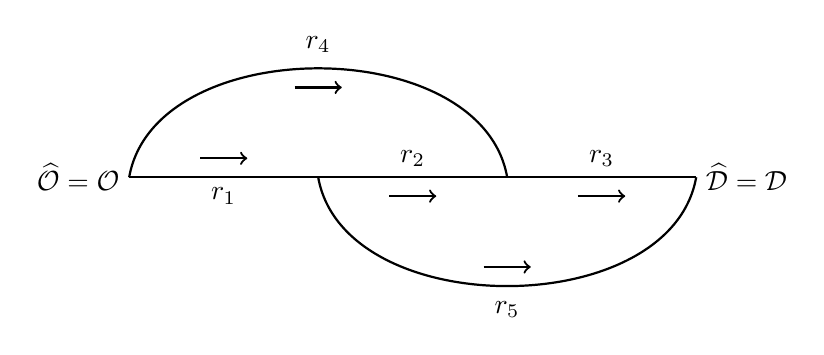
\begin{tikzpicture}[scale=1.2, rotate=-90]

% Nodi principali
\coordinate (A) at (0,0);
\coordinate (B) at (0,6);
\coordinate (Y) at (0,2);
\coordinate (X) at (0,4);

% Segmento principale
\draw[thick] (A) -- (B);

% Arco superiore
\draw[thick]
(B) to[out=-10,in=10] (Y);

% Arco inferiore
\draw[thick]
(A) to[out=170,in=-170] (X);

% Collegamento centrale tratteggiato
\draw[thick, dashed] (Y) -- (X);

% Freccia direzione
\draw[->, thick] (-0.2,0.75) -- (-0.2,1.25);
\draw[->, thick] (0.2,2.75) -- (0.2,3.25);
\draw[->, thick] (0.2,4.75) -- (0.2,5.25);
\draw[->, thick] (-0.95,1.75) -- (-0.95,2.25);
\draw[->, thick] (0.95,3.75) -- (0.95,4.25);

% Etichette
\node[left] at (A) {$\widehat{\mathcal{O}} = \widecheck{\mathcal{O}}$};
\node[right] at (B) {$\widehat{\mathcal{D}} = \widecheck{\mathcal{D}}$};

% Etichette archi
\node at (0.2, 1) {$r_1$};
\node at (-0.2,3) {$r_2$};
\node at (-0.2, 5) {$r_3$};
\node at (-1.4,2) {$r_4$};
\node at (1.4, 4) {$r_5$};

\end{tikzpicture}

\end{figure}

Il percorso $(r_1, r_2, r_3)$ è il percorso principale che, in situazioni di traffico moderato ($\widehat{\zeta}$ e $\widecheck{\zeta}$ non troppo elevati), le due popolazioni utilizzano esclusivamente per arrivare a destinazione.
Le strade $r_4$ e $r_5$ rappresentano, invece, delle "scorciatoie", convenienti solo in caso di traffico intenso ($\widehat{\zeta}$ e $\widecheck{\zeta}$ elevati). L'unico motivo
per cui queste ultime due strade sono opzioni allettanti per i guidatori è la precedenza che i veicoli hanno in uscita da esse: i veicoli provenienti da $r_4$ hanno precedenza sui veicoli
provenienti da $r_2$ (analogo per i veicoli su $r_5$ rispetto a quelli su $r_3$).

Consideriamo apparteneti alla popolazione \textit{hat} i veicoli che conoscono le "scorciatoie" $r_4$ e $r_5$, mentre i veicoli di \textit{check} ne ignorano l'esistenza:

\begin{equation*}
\begin{array}{r @{\hspace{2cm}} r}

\widehat{\gamma}_1 = (r_1, r_2, r_3) &
\widecheck{\gamma}_1 = (r_1, r_2, r_3)\\

\widehat{\gamma}_2 = (r_4, r_3) & \\

\widehat{\gamma}_3 = (r_1, r_5) & \\
$$
\end{array}
\end{equation*}

In una situazione di traffico intenso, quindi, ci aspetteremmo che i guidatori \textit{hat} comincino ad utilizzare esclusivamente le scorciatoie, sfruttando la precedenza
sul percorso principale per evitare il traffico intenso. Definiamo dunque le funzioni di costo:
\begin{equation*}
\begin{array}{r @{\hspace{2cm}} r}

\widehat{\tau}_1(\eta) = 30+\widehat{\eta}+\widecheck{\eta} &
\widecheck{\tau}_1(\eta) = 30+\widehat{\eta}+\widecheck{\eta} \\

\widehat{\tau}_2(\eta) = 30+\widehat{\eta}+\widecheck{\eta} &
\widecheck{\tau}_2(\eta) = 30+\widehat{\eta}+\widecheck{\eta} \\

\widehat{\tau}_3(\eta) = 5+\widehat{\eta}+\widecheck{\eta} &
\widecheck{\tau}_3(\eta) = 5+\widehat{\eta}+\widecheck{\eta} \\

\widehat{\tau}_4(\eta) = 135+\widehat{\eta} &
\widecheck{\tau}_4(\eta) =  +\infty\\

\widehat{\tau}_5(\eta) = 105+\widehat{\eta} &
\widecheck{\tau}_5(\eta) = +\infty 
$$
\end{array}
\end{equation*}
Ed otteniamo:

Facendo ciò, però, si otterrà un peggioramento nel tempo di attraversamento della rete per la popolazione \textit{check}
(dato che i guidatori \text{check} sono costretti a cedere la precedenza), già elevato a causa dell'elevata presenza di veicoli nella rete. Aumentando, dunque, il costo delle
due scorciatoie si dovrebbe ottenere un miglioramento nel tempo di percorrenza della rete per \textit{check}.